\section{\large Технологическая часть}

В  данном  разделе  рассмотрены  средства  разработки  программного
обеспечения, приведены детали реализации и листинги исходных кодов, описан интерфейс разработанной программы и приведена демонстрация работы.

Приведённые листинги исходных кодов включают в себя создание таблиц и ограничений, создание ролевой модели и функции управления доступами (на основе приведённой выше диаграммы вариантов использования).

\subsection{Средства реализации}
Как  основное  средство  реализации  и  разработки  ПО  был  выбран  язык программирования  TypeScript \cite{ts}.
Причиной  выбора  данного  языка  является  тот факт,  что  он  имеет компилируется в JavaScript \cite{js}, что делает его также кроссплатформенным и позволяет использовать библиотеки, написанные для JavaScript.
Наличие типизации позволяет траспилятору получать более эффективный код, чем для JavaScript, вследствие чего производительность TypeScript является предпочтительнее при написании сервера \cite{ts-vs-js}.

В качестве СУБД будет выбрана PostgreSQL~\cite{postgres}, поскольку она является системой с открытым исходным кодом, одновременно имея большую пользовательскую базу (является четвёртой по популярности СУБД, становится более популярной~\cite{db-engine}, в то время как Oracle не только является проприетарной системой, но и не действует на территории РФ. 

Для запуска написанного сервера была использована библиотека Node.js \cite{nodejs} для языка JavaScript, которая предоставляет асинхронное окружение, что позволяет избавиться от синхронности и разрабатывать более производительные приложения.

Для обработки HTTP запросов была использована библиотека Fastify \cite{fastify}, которая была выбрана из-за своего превосходства в скорости обработки соединений по сравнению с другими библиотеками (Koa, Express, Restify, Hapi) \cite{fastify-b}.
Для доступа к СУБД, реализованной при помощи PostgreSQL, была использована библиотека pg-promise~\cite{pg-promise}, предоставляющая интерфейс для взаимодействия с базой данных.

Для реализации графического интерфейса API была использована библиотека FastAPI~\cite{fastapi}, позволяющая быстро создать рабочий интерфейс для созданного API (вместе с документацией).
Средой разработки  послужил  графический  редактор  Visual  Studio  Code~\cite{vscode},  который известен  содержанием  большого  количество  плагинов,  ускоряющих  процесс разработки  программы.


\subsubsection{Создание таблиц и ограничений}

Скрипт создания пользовательских типов данных приведён на листинге~\ref{code:usertypes}. 

\begin{code}
	\captionsetup{justification=centering}
	\captionof{listing}{Определение пользовательских типов данных}
	\label{code:usertypes}
	\inputminted
	[
	frame=single,
	framerule=0.5pt,
	framesep=20pt,
	fontsize=\small,
	tabsize=4,
	linenos,
	numbersep=5pt,
	xleftmargin=10pt,
	]
	{text}
	{/home/paul/Desktop/reps/bmstu-db-cw/docs/code/usertypes.sql}
\end{code}

<<<<<<< Updated upstream
На листинге \ref{code:createtables1} приведён пример скрипта создания таблицы пациентов (скрипты для создания остальных таблиц были созданы аналогично).
\clearpage

=======

\begin{code}
	\captionsetup{justification=centering}
	\captionof{listing}{Создание таблиц (часть 1)}
	\label{code:createtables1}
	\inputminted
	[
	frame=single,
	framerule=0.5pt,
	framesep=20pt,
	fontsize=\small,
	tabsize=4,
	linenos,
	numbersep=5pt,
	xleftmargin=10pt,
	]
	{text}
	{/home/paul/Desktop/reps/bmstu-db-cw/docs/code/createtables1.sql}
\end{code}

\clearpage

\begin{figure}[H]
\begin{code}
	\captionsetup{justification=centering}
	\captionof{listing}{Создание таблиц (часть 2)}
	\label{code:createtables2}
	\inputminted
	[
	frame=single,
	framerule=0.5pt,
	framesep=20pt,
	fontsize=\small,
	tabsize=4,
	linenos,
	numbersep=5pt,
	xleftmargin=10pt,
	]
	{text}
	{/home/paul/Desktop/reps/bmstu-db-cw/docs/code/createtables2.sql}
\end{code}
\end{figure}

\clearpage
>>>>>>> Stashed changes

\begin{code}
	\captionsetup{justification=centering}
<<<<<<< Updated upstream
	\captionof{listing}{Создание таблицы пациентов}
	\label{code:createtables1}
=======
	\captionof{listing}{Создание таблиц (часть 3)}
	\label{code:createtables3}
	\inputminted
	[
	frame=single,
	framerule=0.5pt,
	framesep=20pt,
	fontsize=\small,
	tabsize=4,
	linenos,
	numbersep=5pt,
	xleftmargin=10pt,
	]
	{text}
	{/home/paul/Desktop/reps/bmstu-db-cw/docs/code/createtables3.sql}
\end{code}
\end{figure}

\begin{figure}[H]
\begin{code}
	\captionsetup{justification=centering}
	\captionof{listing}{Создание таблиц (часть 4)}
	\label{code:createtables4}
	\inputminted
	[
	frame=single,
	framerule=0.5pt,
	framesep=20pt,
	fontsize=\small,
	tabsize=4,
	linenos,
	numbersep=5pt,
	xleftmargin=10pt,
	]
	{text}
	{/home/paul/Desktop/reps/bmstu-db-cw/docs/code/createtables4.sql}
\end{code}
\end{figure}

\begin{figure}[H]
\begin{code}
	\captionsetup{justification=centering}
	\captionof{listing}{Создание таблиц (часть 5)}
	\label{code:createtables5}
>>>>>>> Stashed changes
	\inputminted
	[
	frame=single,
	framerule=0.5pt,
	framesep=20pt,
	fontsize=\small,
	tabsize=4,
	linenos,
	numbersep=5pt,
	xleftmargin=10pt,
	]
	{text}
<<<<<<< Updated upstream
	{/Users/p.kalashkov/Desktop/sixthTerm/bmstu-db-cw/docs/code/createtables1.sql}
=======
	{/home/paul/Desktop/reps/bmstu-db-cw/docs/code/createtables5.sql}
>>>>>>> Stashed changes
\end{code}
%
%\clearpage
%
%\begin{figure}[H]
%\begin{code}
%	\captionsetup{justification=centering}
%	\captionof{listing}{Создание таблиц (часть 2)}
%	\label{code:createtables2}
%	\inputminted
%	[
%	frame=single,
%	framerule=0.5pt,
%	framesep=20pt,
%	fontsize=\small,
%	tabsize=4,
%	linenos,
%	numbersep=5pt,
%	xleftmargin=10pt,
%	]
%	{text}
%	{/Users/p.kalashkov/Desktop/sixthTerm/bmstu-db-cw/docs/code/createtables2.sql}
%\end{code}
%\end{figure}
%
%\clearpage
%
%\begin{figure}[H]
%\begin{code}
%	\captionsetup{justification=centering}
%	\captionof{listing}{Создание таблиц (часть 3)}
%	\label{code:createtables3}
%	\inputminted
%	[
%	frame=single,
%	framerule=0.5pt,
%	framesep=20pt,
%	fontsize=\small,
%	tabsize=4,
%	linenos,
%	numbersep=5pt,
%	xleftmargin=10pt,
%	]
%	{text}
%	{/Users/p.kalashkov/Desktop/sixthTerm/bmstu-db-cw/docs/code/createtables3.sql}
%\end{code}
%\end{figure}
%
%\begin{figure}[H]
%\begin{code}
%	\captionsetup{justification=centering}
%	\captionof{listing}{Создание таблиц (часть 4)}
%	\label{code:createtables4}
%	\inputminted
%	[
%	frame=single,
%	framerule=0.5pt,
%	framesep=20pt,
%	fontsize=\small,
%	tabsize=4,
%	linenos,
%	numbersep=5pt,
%	xleftmargin=10pt,
%	]
%	{text}
%	{/Users/p.kalashkov/Desktop/sixthTerm/bmstu-db-cw/docs/code/createtables4.sql}
%\end{code}
%\end{figure}
%
%\begin{figure}[H]
%\begin{code}
%	\captionsetup{justification=centering}
%	\captionof{listing}{Создание таблиц (часть 5)}
%	\label{code:createtables5}
%	\inputminted
%	[
%	frame=single,
%	framerule=0.5pt,
%	framesep=20pt,
%	fontsize=\small,
%	tabsize=4,
%	linenos,
%	numbersep=5pt,
%	xleftmargin=10pt,
%	]
%	{text}
%	{/Users/p.kalashkov/Desktop/sixthTerm/bmstu-db-cw/docs/code/createtables5.sql}
%\end{code}
%\end{figure}

Также в созданные таблицы необходимо добавить ограничения. На листинге~\ref{code:constraints1} приведён пример запроса, создающего ограничение для таблицы пациентов (для остальлных таблиц команды аналогичны).

\begin{code}
	\captionsetup{justification=centering}
	\captionof{listing}{Создание ограничений для таблицы пациентов}
	\label{code:constraints1}
	\inputminted
	[
	frame=single,
	framerule=0.5pt,
	framesep=20pt,
	fontsize=\small,
	tabsize=4,
	linenos,
	numbersep=5pt,
	xleftmargin=10pt,
	]
	{text}
	{/home/paul/Desktop/reps/bmstu-db-cw/docs/code/constraints1.sql}
\end{code}
%
%\clearpage
%
%\begin{figure}[H]
%\begin{code}
%	\captionsetup{justification=centering}
%	\captionof{listing}{Создание ограничений для созданных таблиц (часть 2)}
%	\label{code:constraints2}
%	\inputminted
%	[
%	frame=single,
%	framerule=0.5pt,
%	framesep=20pt,
%	fontsize=\small,
%	tabsize=4,
%	linenos,
%	numbersep=5pt,
%	xleftmargin=10pt,
%	]
%	{text}
%	{/Users/p.kalashkov/Desktop/sixthTerm/bmstu-db-cw/docs/code/constraints2.sql}
%\end{code}
%\end{figure}
%
%\clearpage
%
%\begin{figure}[H]
%\begin{code}
%	\captionsetup{justification=centering}
%	\captionof{listing}{Создание ограничений для созданных таблиц (часть 3)}
%	\label{code:constraints3}
%	\inputminted
%	[
%	frame=single,
%	framerule=0.5pt,
%	framesep=20pt,
%	fontsize=\small,
%	tabsize=4,
%	linenos,
%	numbersep=5pt,
%	xleftmargin=10pt,
%	]
%	{text}
%	{/Users/p.kalashkov/Desktop/sixthTerm/bmstu-db-cw/docs/code/constraints3.sql}
%\end{code}
%\end{figure}

\subsubsection{Создание ролевой модели и управление доступами}

<<<<<<< Updated upstream
На основе приведённой выше диаграммы вариантов использования создадим роли и распределим доступы к таблицам.

\clearpage

=======
\begin{figure}[H]
\begin{code}
	\captionsetup{justification=centering}
	\captionof{listing}{Создание ограничений для созданных таблиц (часть 2)}
	\label{code:constraints2}
	\inputminted
	[
	frame=single,
	framerule=0.5pt,
	framesep=20pt,
	fontsize=\small,
	tabsize=4,
	linenos,
	numbersep=5pt,
	xleftmargin=10pt,
	]
	{text}
	{/home/paul/Desktop/reps/bmstu-db-cw/docs/code/constraints2.sql}
\end{code}
\end{figure}

\clearpage

\begin{figure}[H]
\begin{code}
	\captionsetup{justification=centering}
	\captionof{listing}{Создание ограничений для созданных таблиц (часть 3)}
	\label{code:constraints3}
	\inputminted
	[
	frame=single,
	framerule=0.5pt,
	framesep=20pt,
	fontsize=\small,
	tabsize=4,
	linenos,
	numbersep=5pt,
	xleftmargin=10pt,
	]
	{text}
	{/home/paul/Desktop/reps/bmstu-db-cw/docs/code/constraints3.sql}
\end{code}
\end{figure}

\subsubsection{Создание ролевой модели и управление доступами}

На основе приведённой выше Use-Case диаграммы создадим роли и распределим доступы к таблицам.

>>>>>>> Stashed changes
\begin{code}
	\captionsetup{justification=centering}
	\captionof{listing}{Создание ролей}
	\label{code:roles1}
	\inputminted
	[
	frame=single,
	framerule=0.5pt,
	framesep=20pt,
	fontsize=\small,
	tabsize=4,
	linenos,
	numbersep=5pt,
	xleftmargin=10pt,
	]
	{text}
	{/home/paul/Desktop/reps/bmstu-db-cw/docs/code/roles1.sql}
\end{code}

\begin{code}
	\captionsetup{justification=centering}
	\captionof{listing}{Распределение доступов между ролями (часть 1)}
	\label{code:roles2}
	\inputminted
	[
	frame=single,
	framerule=0.5pt,
	framesep=20pt,
	fontsize=\small,
	tabsize=4,
	linenos,
	numbersep=5pt,
	xleftmargin=10pt,
	]
	{text}
	{/home/paul/Desktop/reps/bmstu-db-cw/docs/code/roles2.sql}
\end{code}

\begin{figure}[H]
\begin{code}
	\captionsetup{justification=centering}
	\captionof{listing}{Распределение доступов между ролями (часть 2)}
	\label{code:roles3}
	\inputminted
	[
	frame=single,
	framerule=0.5pt,
	framesep=20pt,
	fontsize=\small,
	tabsize=4,
	linenos,
	numbersep=5pt,
	xleftmargin=10pt,
	]
	{text}
	{/home/paul/Desktop/reps/bmstu-db-cw/docs/code/roles3.sql}
\end{code}
\end{figure}

Для управления доступами для конкретных соединений была использована технология политики RLS (\textit{англ.} Row Level Security Polices) и процедура, приведённая на листингах \ref{code:roles4} -- \ref{code:roles5}.

\begin{code}
	\captionsetup{justification=centering}
	\captionof{listing}{Управление доступами при помощи RLS (часть 1)}
	\label{code:roles4}
	\inputminted
	[
	frame=single,
	framerule=0.5pt,
	framesep=20pt,
	fontsize=\small,
	tabsize=4,
	linenos,
	numbersep=5pt,
	xleftmargin=10pt,
	]
	{text}
	{/home/paul/Desktop/reps/bmstu-db-cw/docs/code/roles4.sql}
\end{code}

\begin{figure}[H]
\begin{code}
	\captionsetup{justification=centering}
	\captionof{listing}{Управление доступами при помощи RLS (часть 2)}
	\label{code:roles5}
	\inputminted
	[
	frame=single,
	framerule=0.5pt,
	framesep=20pt,
	fontsize=\small,
	tabsize=4,
	linenos,
	numbersep=5pt,
	xleftmargin=10pt,
	]
	{text}
	{/home/paul/Desktop/reps/bmstu-db-cw/docs/code/roles5.sql}
\end{code}
\end{figure}

%\begin{figure}[H]
%\begin{code}
%	\captionsetup{justification=centering}
%	\captionof{listing}{Управление доступами при помощи RLS (часть 3)}
%	\label{code:roles6}
%	\inputminted
%	[
%	frame=single,
%	framerule=0.5pt,
%	framesep=20pt,
%	fontsize=\small,
%	tabsize=4,
%	linenos,
%	numbersep=5pt,
%	xleftmargin=10pt,
%	]
%	{text}
%	{/Users/p.kalashkov/Desktop/sixthTerm/bmstu-db-cw/docs/code/roles6.sql}
%\end{code}
%\end{figure}


%\subsection{Реализация сервера}
%
%В  расположенных  ниже  листингах \ref{code:1-1} -- \ref{code:2-3} приведены реализации менеджера соединений и класса соединения, объекты которого используются в обработчиках запросов.
%\clearpage
%
%\begin{figure}[H]
%\begin{code}
%	\captionsetup{justification=centering}
%	\captionof{listing}{Реализация менеджера соединений (часть 1)}
%	\label{code:1-1}
%	\inputminted
%	[
%	frame=single,
%	framerule=0.5pt,
%	framesep=20pt,
%	fontsize=\small,
%	tabsize=4,
%	linenos,
%	numbersep=5pt,
%	xleftmargin=10pt,
%	]
%	{text}
%	{code/ConnectManager1.ts}
%\end{code}
%\end{figure}
%
%\clearpage
%
%\begin{figure}[H]
%\begin{code}
%	\captionsetup{justification=centering}
%	\captionof{listing}{Реализация менеджера соединений (часть 2)}
%	\label{code:1-2}
%	\inputminted
%	[
%	frame=single,
%	framerule=0.5pt,
%	framesep=20pt,
%	fontsize=\small,
%	tabsize=4,
%	linenos,
%	numbersep=5pt,
%	xleftmargin=10pt,
%	]
%	{text}
%	{code/ConnectManager2.ts}
%\end{code}
%\end{figure}
%
%\begin{code}
%	\captionsetup{justification=centering}
%	\captionof{listing}{Реализация класса соединения (часть 1)}
%	\label{code:2-1}
%	\inputminted
%	[
%	frame=single,
%	framerule=0.5pt,
%	framesep=20pt,
%	fontsize=\small,
%	tabsize=4,
%	linenos,
%	numbersep=5pt,
%	xleftmargin=10pt,
%	]
%	{text}
%	{code/Connection1.ts}
%\end{code}
%
%\begin{figure}[H]
%\begin{code}
%	\captionsetup{justification=centering}
%	\captionof{listing}{Реализация класса соединения (часть 2)}
%	\label{code:2-2}
%	\inputminted
%	[
%	frame=single,
%	framerule=0.5pt,
%	framesep=20pt,
%	fontsize=\small,
%	tabsize=4,
%	linenos,
%	numbersep=5pt,
%	xleftmargin=10pt,
%	]
%	{text}
%	{code/Connection2.ts}
%\end{code}
%\end{figure}
%
%\begin{figure}[H]
%\begin{code}
%	\captionsetup{justification=centering}
%	\captionof{listing}{Реализация класса соединения (часть 3)}
%	\label{code:2-3}
%	\inputminted
%	[
%	frame=single,
%	framerule=0.5pt,
%	framesep=20pt,
%	fontsize=\small,
%	tabsize=4,
%	linenos,
%	numbersep=5pt,
%	xleftmargin=10pt,
%	]
%	{text}
%	{code/Connection2.ts}
%\end{code}
%\end{figure}

\subsection{Описание интерфейса}

В основной части страницы находятся методы API, а также их особенности (тип метода, адрес методы, структура, которую метод использует). Часть таких методов приведена на рисунке \ref{fig:interface-1}). 
\begin{figure}[h]
	\centering
	\captionsetup{justification=centering}
<<<<<<< Updated upstream
	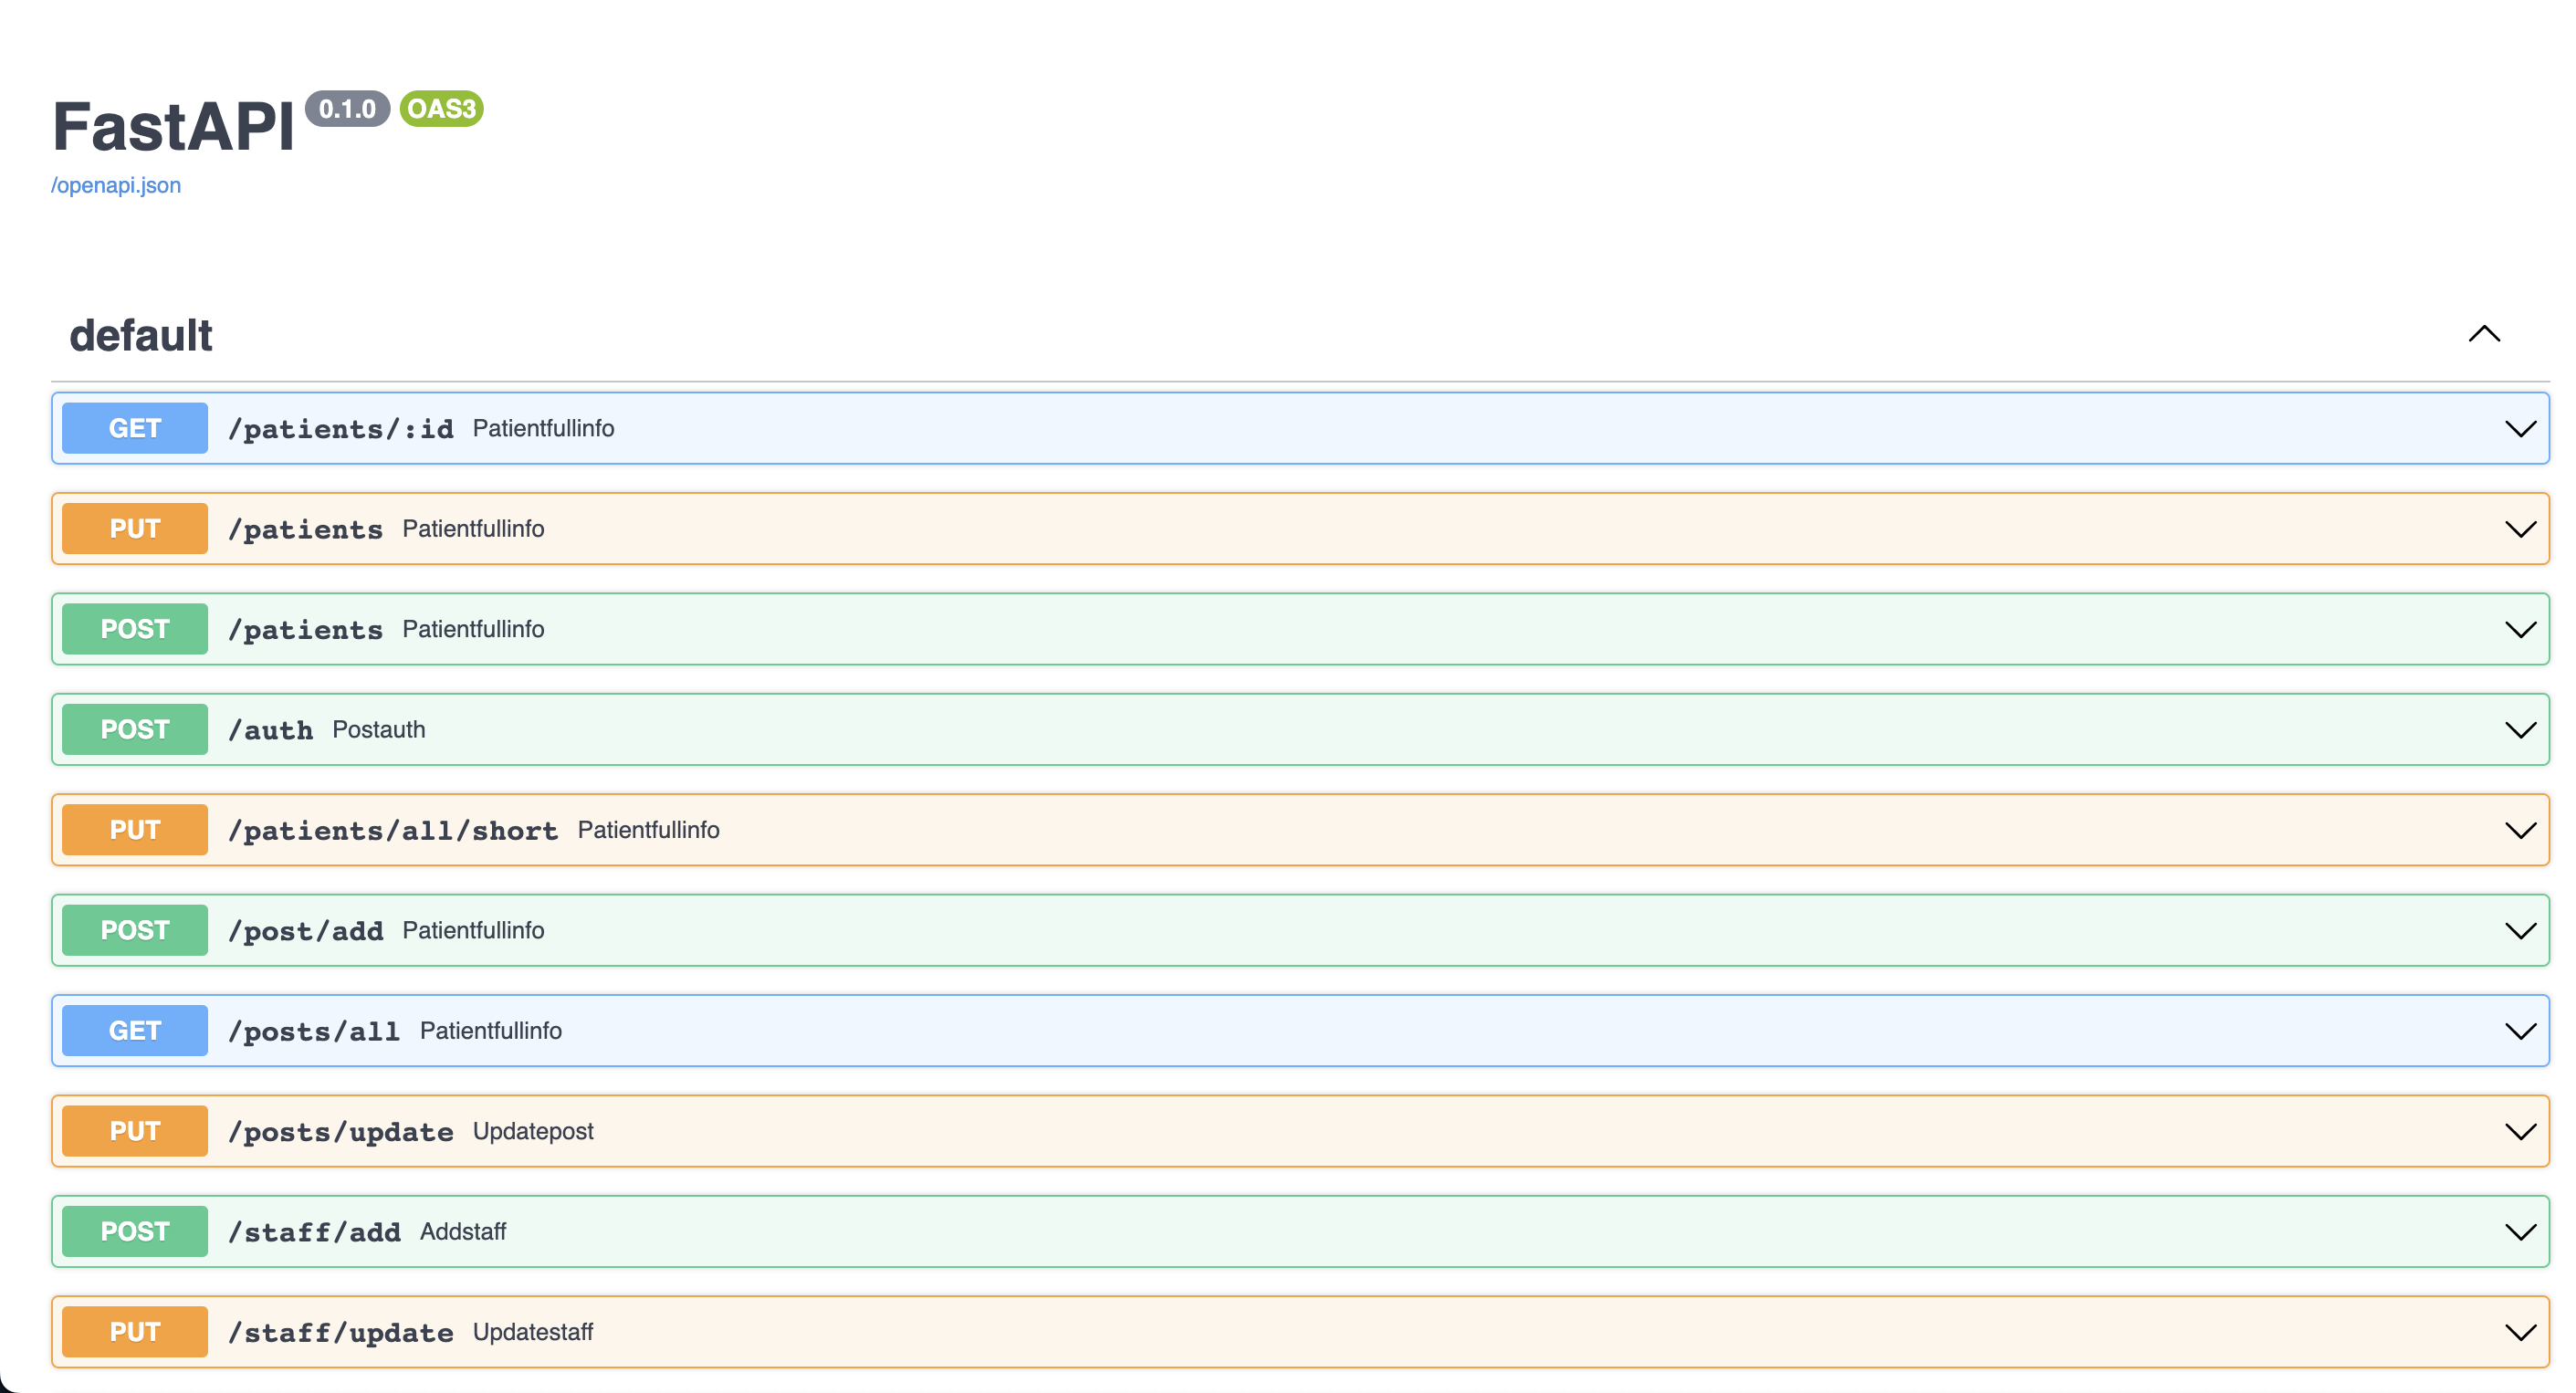
\includegraphics[width=170mm]{img/interface.png}
	\caption{Интерфейс программы: методы API}
	\label{fig:interface-1}
=======
	\captionof{listing}{Управление доступами при помощи RLS (часть 3)}
	\label{code:roles6}
	\inputminted
	[
	frame=single,
	framerule=0.5pt,
	framesep=20pt,
	fontsize=\small,
	tabsize=4,
	linenos,
	numbersep=5pt,
	xleftmargin=10pt,
	]
	{text}
	{/home/paul/Desktop/reps/bmstu-db-cw/docs/code/roles6.sql}
\end{code}
>>>>>>> Stashed changes
\end{figure}

По нажатию на элемент каждого метода появляется подробное описание: какие данные метод принимает на вход, какие параметры являются обязательными, а какие опциональными, структуры какого вида возвращает и в каком виде, что возвращает в случае ошибки (рисунок \ref{fig:interface-2}).
\begin{figure}[h]
	\centering
	\captionsetup{justification=centering}
	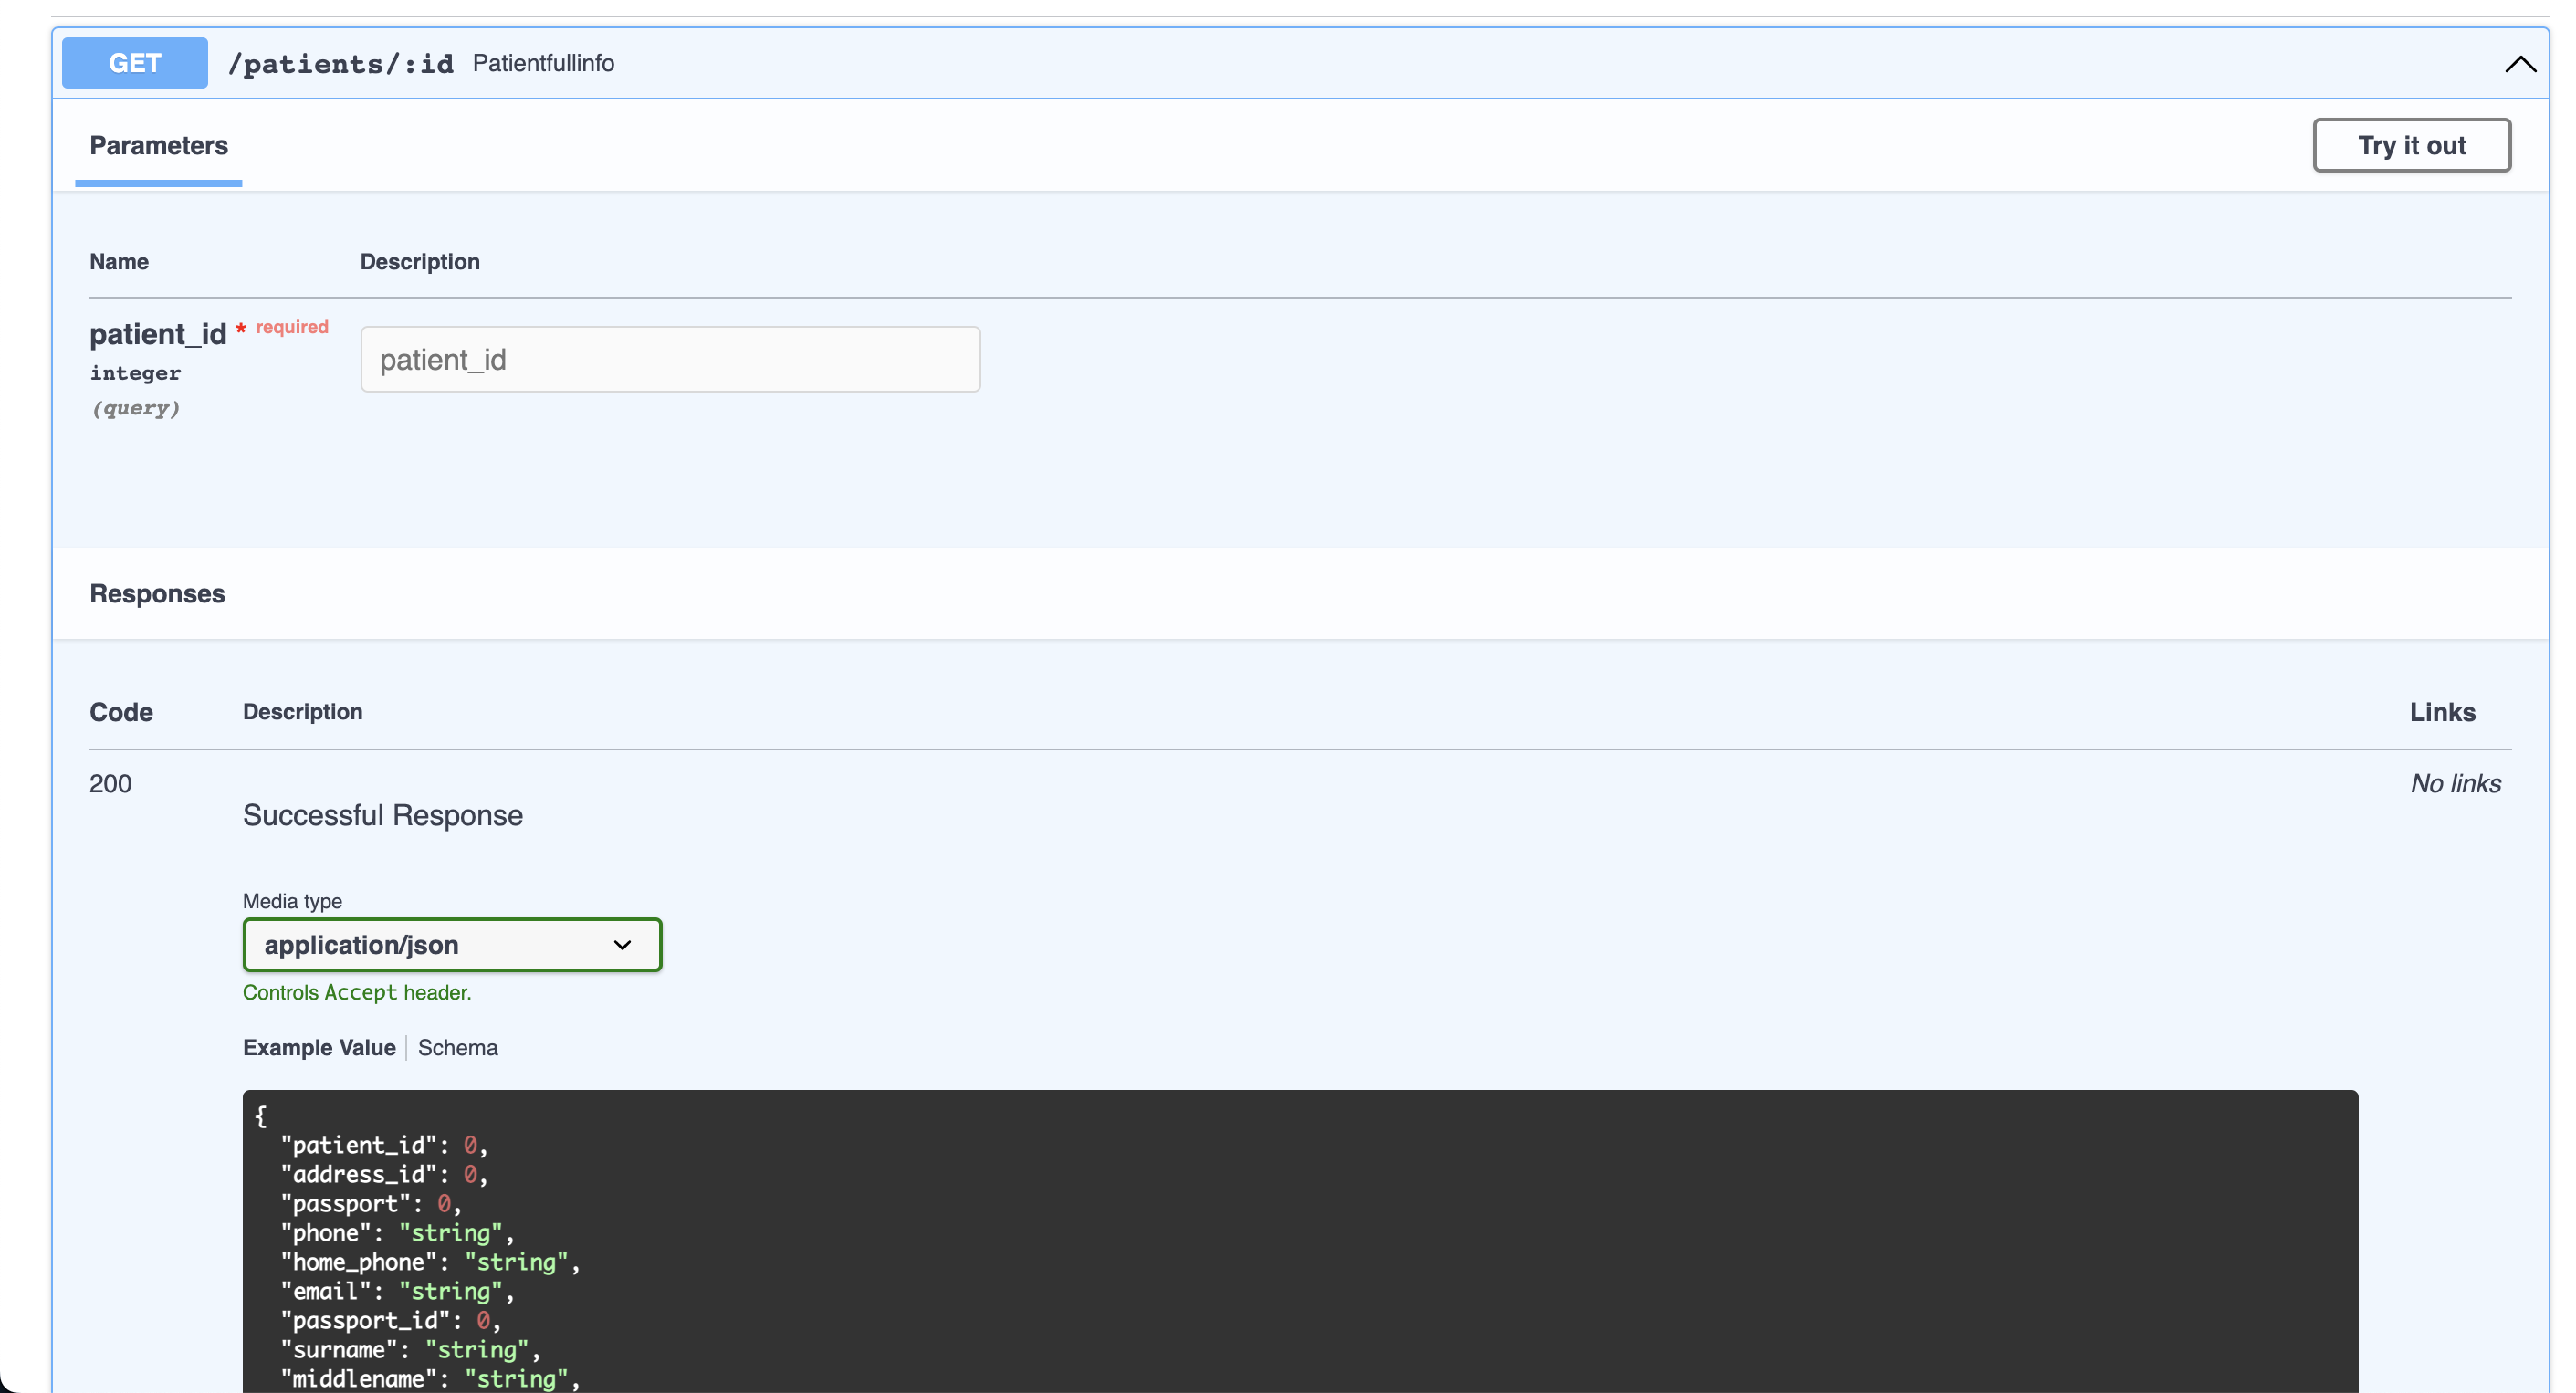
\includegraphics[width=170mm]{img/interface-2.png}
	\caption{Интерфейс программы: подробное описание метода API}
	\label{fig:interface-2}
\end{figure}


\subsection{Демонстрация работы программы}

На рисунках \ref{fig:example-1} -- \ref{fig:example-2} продемонстрирована работа программы на примере осуществления запроса для получения списка пациентов. Созданный интерфейс позволяет не только просматривать методы API, как было показано выше, но и осуществлять отправку конкретных запросов.
При этом имеется возможность посмотреть результат запроса (его статус и заголовки, присланные данные), его адрес, а также получить команды для отправления эквивалентного запроса из командной строки.

\clearpage

\begin{figure}[h]
	\centering
	\captionsetup{justification=centering}
	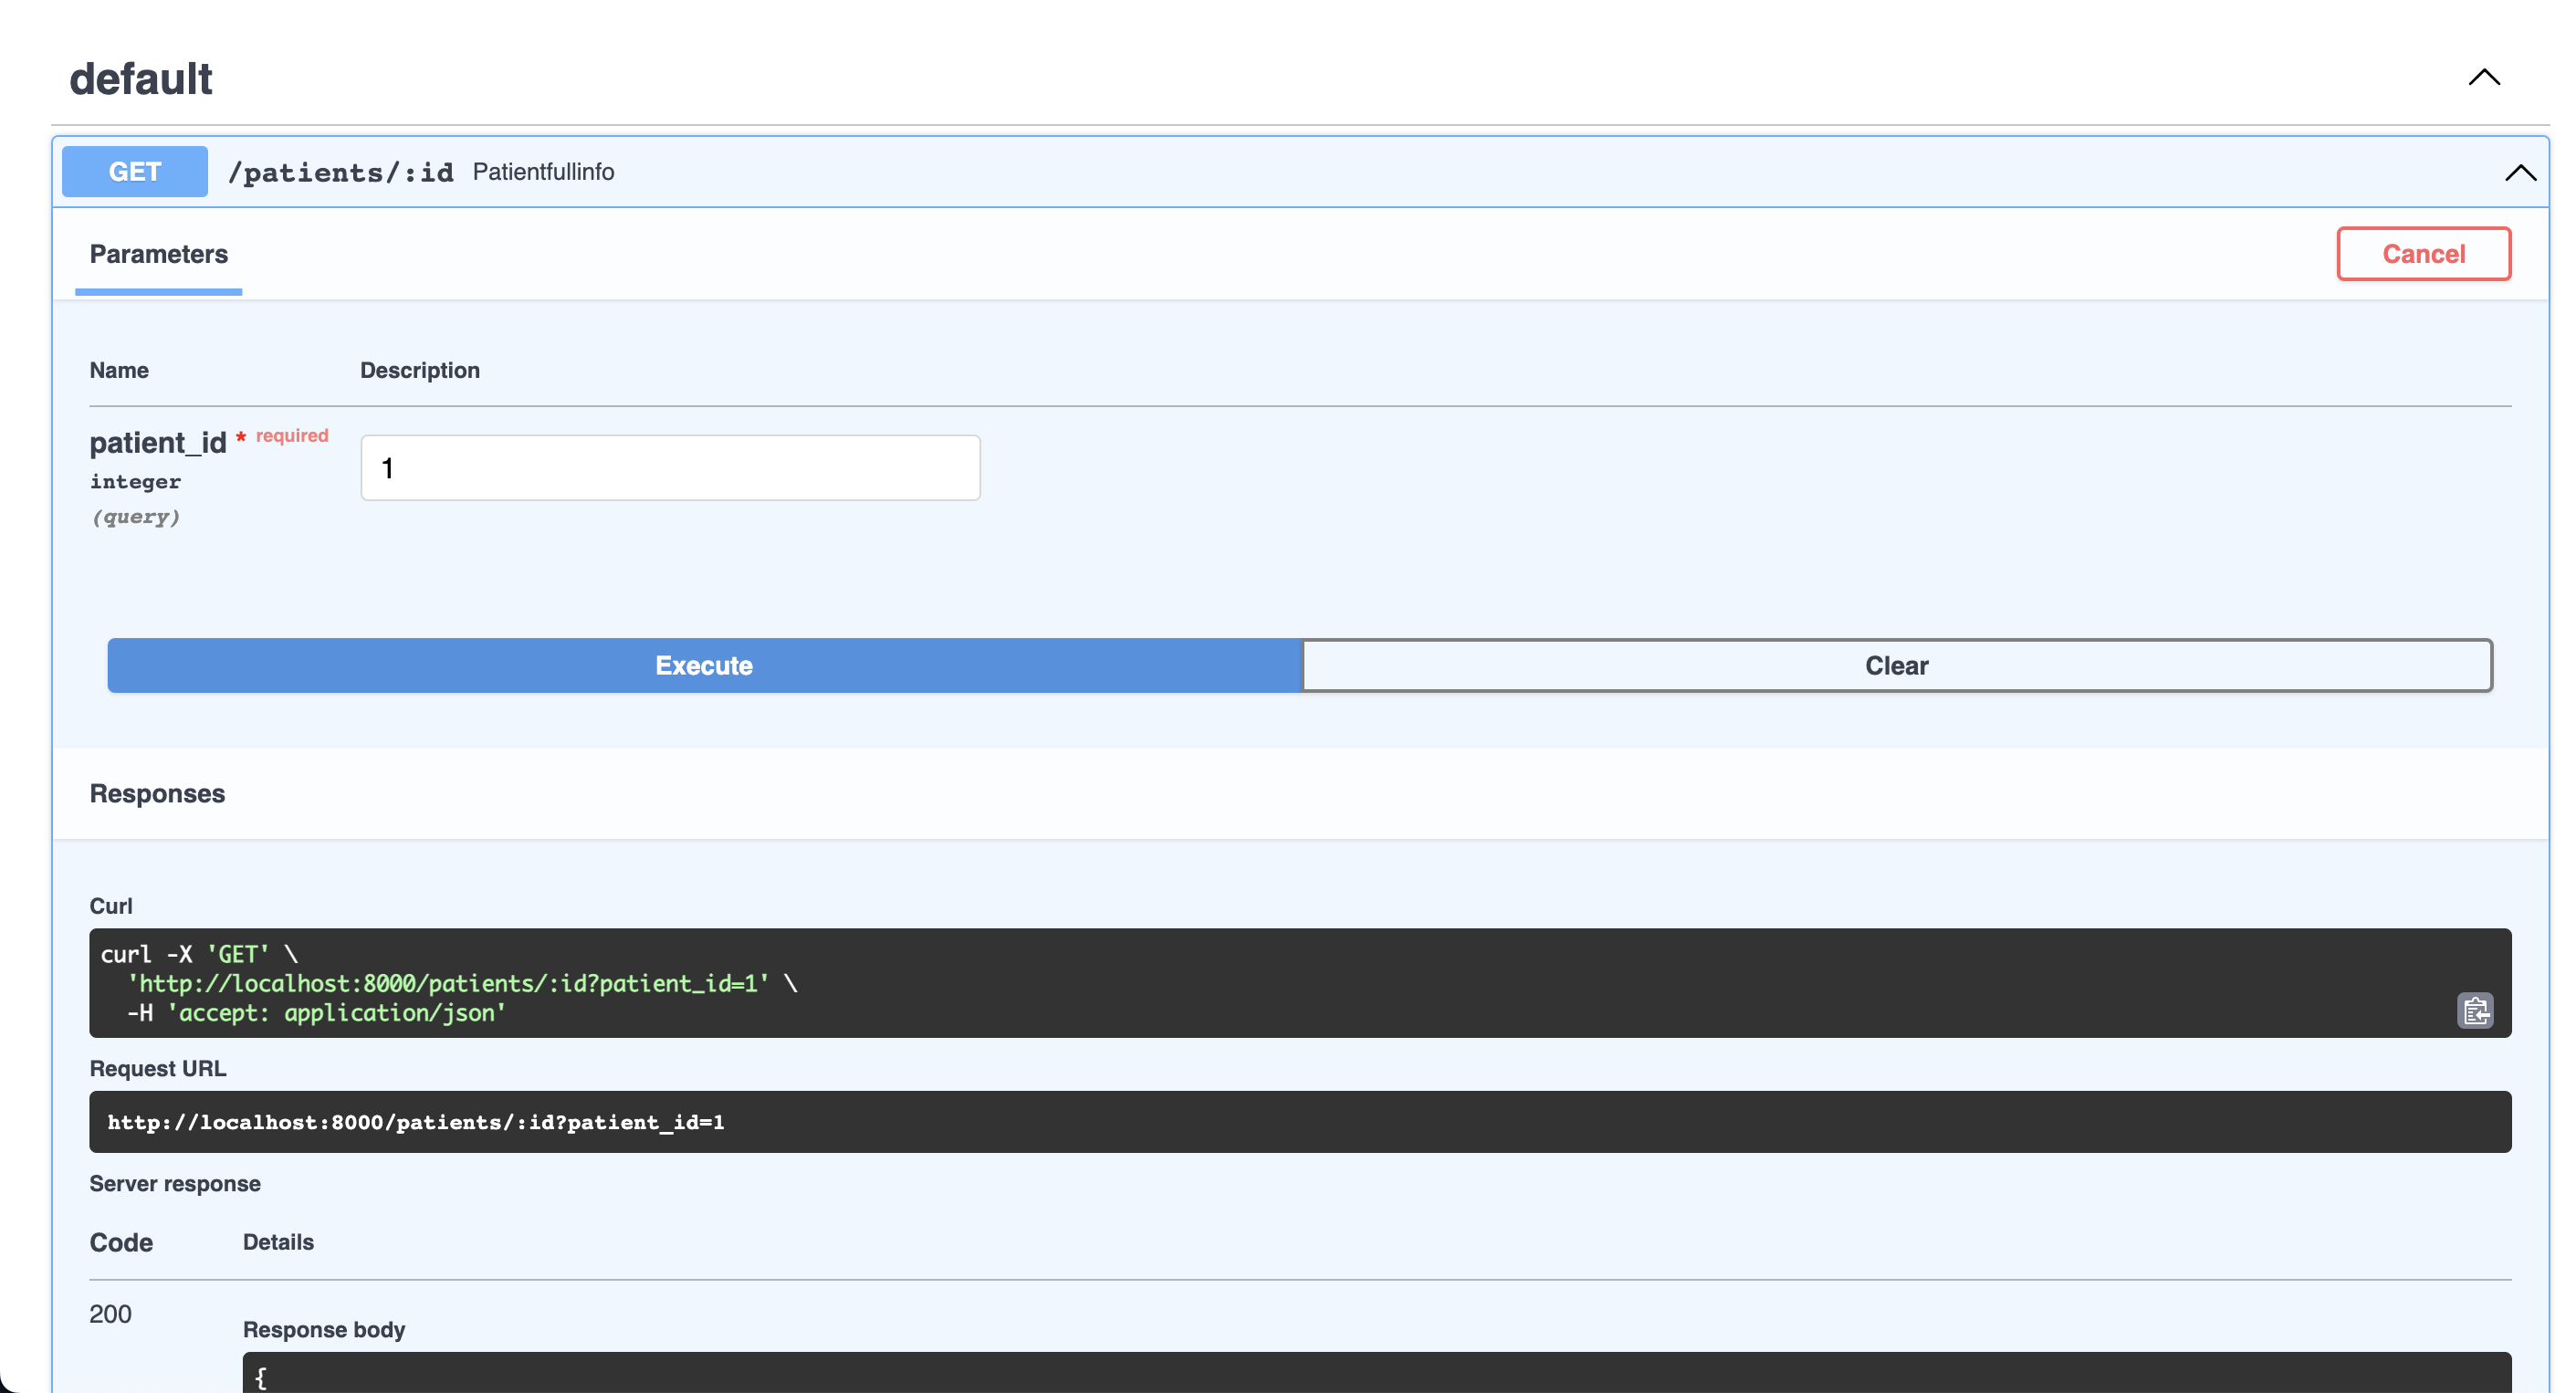
\includegraphics[width=152mm]{img/example-1.png}
	\caption{Демонстрация  работы  программы  (часть 1)}
	\label{fig:example-1}
\end{figure}

\begin{figure}[h]
	\centering
	\captionsetup{justification=centering}
 	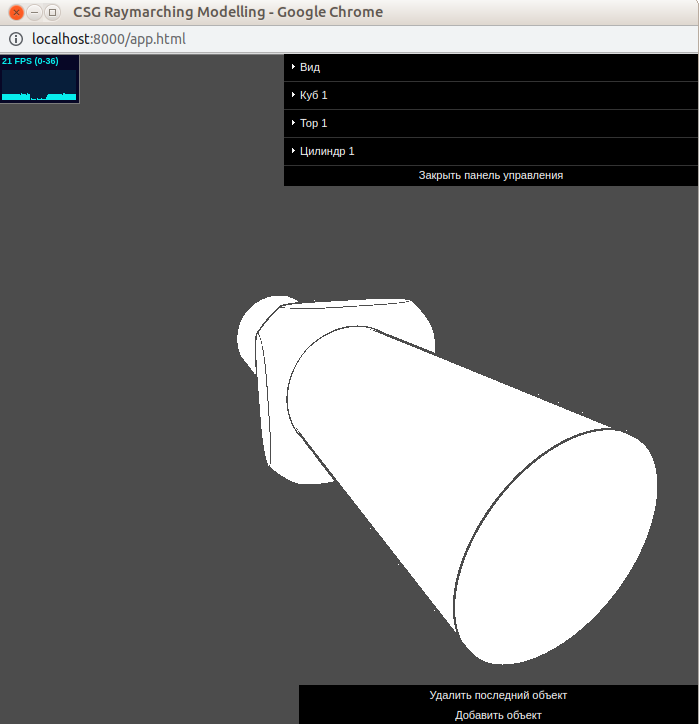
\includegraphics[width=152mm]{img/example-2.png}
	\caption{Демонстрация  работы  программы  (часть 2)}
	\label{fig:example-2}
\end{figure}


\subsection*{Вывод}
В данном разделе были рассмотрены средства реализации ПО, приведены примеры
листинги скриптов создания таблиц и ограничений. Был описан интерфейс разработанной программы, а также приведена демонсстрация работы на примере запроса для получения списка пациентов.
\pagebreak